% указываем класс документа
\documentclass[12pt,a4paper,openany]{extarticle}
% подключаем собственный стилевой файл
\usepackage{mystyle}
% указываем язык (для автоматической вставки слов, типа "Глава", "Содержание", "Литература", "рис." и пр.
\selectlanguage{russian}
\graphicspath{{./images/}}
\usepackage[pdftex]{lscape}

\begin{document}

\part*{Лабораторная работа №5\\
Робот с дифференциальным приводом}

\section{Методические рекомендации}
\hspace*{\parindent}До начала работы студент должен выполнить предыдущие лабораторные этого цикла.

\section{Теоретические сведения}
\hspace*{\parindent}В прошлой работе вы успели познакомиться c таким приемом управления, как ПИД-регулятор. Путем его реализации вам удалось реализовать процесс движения вдоль стены с минимальной ошибкой управления. В данной лабораторной работе будет предложено создать алгоритм движения широко используемого робота с дифференциальным приводом в заданную точку. Такой вид конструкции робота предполагает достаточно большую подвижность и мобильность вкупе со сравнительно легкой математической моделью. 

В робототехнике широко применяется два способа локализации, т.е нахождения координат устройства.

\begin{itemize}
\item Глобальный - получение абсолютных координат робота. Например, GPS
\item Локальный - получение координат робота, относительно какой-либо точки. Например, центра комнаты.
\end{itemize}

В нашем случае модель робота EV3 будет работать в система координат, которая строится каждый раз заново в точке, где на роботе запускается программа.

\paragraph*{Модель робота}$\phantom{-}$\\
\begin{figure}[h!]
	\centering{ 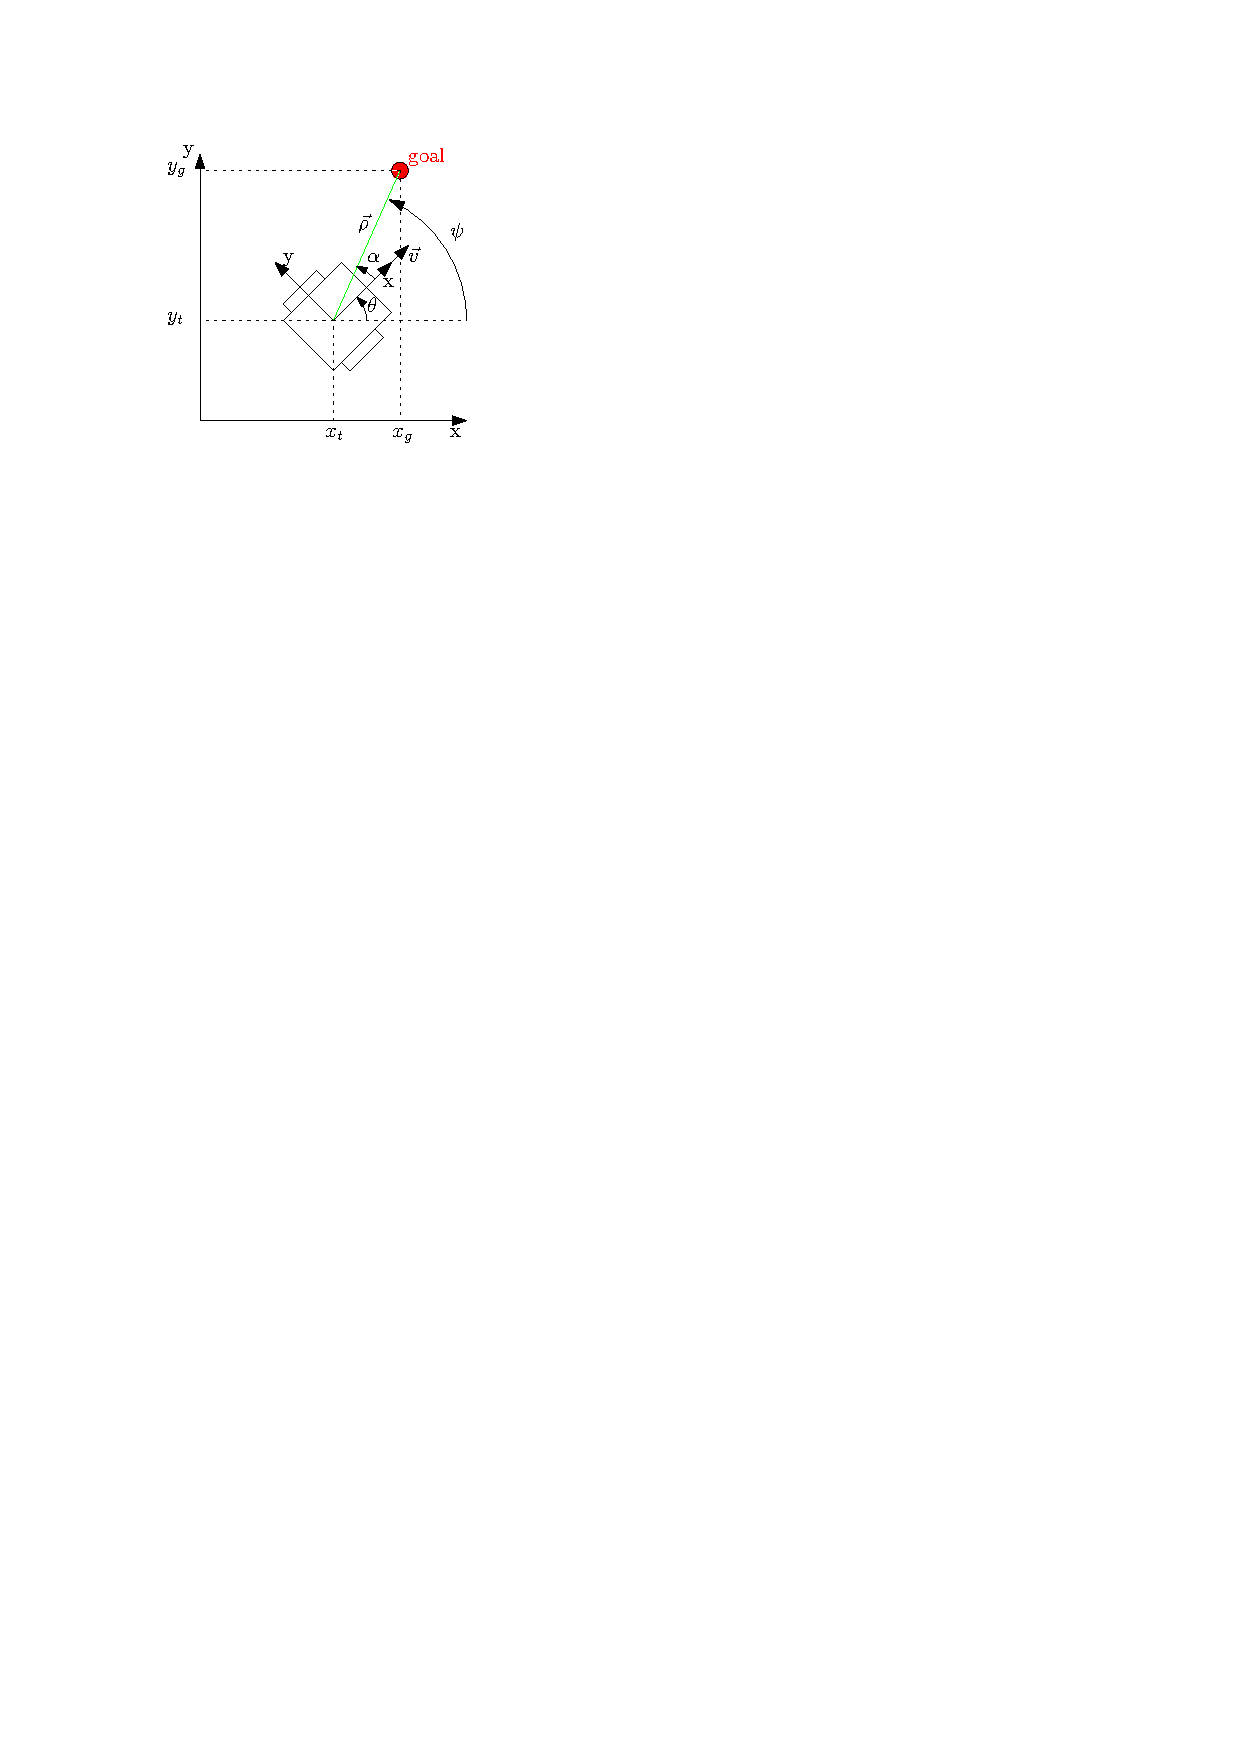
\includegraphics[width = 7cm]{model.pdf} }
	\vspace{1cm}
	\caption{Модель робота.}
	\label{fig:model}
\end{figure}

\hspace*{\parindent} Математическая модель, описывающая робота, всегда делится на две составляющие: динамическую и кинематическую. В динамической моделе учитываются всевозможные динамические показатели системы, такие как момент, сила и т.д. В кинематике рассматривается математика движения, без учета каких-либо сил. В данной работе мы рассмотрим только лишь кинематическую модель, что позволит нам углубиться в решение проблемы оптимального контроля.


Введем некоторые важные величины.

$\vec{\rho} = \begin{pmatrix}x_g - x_t & y_g - y_t\end{pmatrix}$- Расстояние от робота до целевой точки,

$\theta$ - Угол между роботом и базовой осью ох (Курс)

$\psi = \arctan \frac{y_g - y_t}{x_g - x_t}$ - Угол между целевой точкой и курсом робота

$\alpha = \psi - \theta$ - Курсовой угол. Разность между азимутом и курсом робота.

$\vec{v}$ - Линейная скорость робота.

Данная конструкция робота предполагает следующую систему уравнений, которая полностью описывает его движение:

\begin{equation}
 \begin{cases}
	\dot{x} = \cos{\theta} \cdot \frac{\omega_1 + \omega_2}{2}R\\
	\dot{y} = \sin{\theta} \cdot \frac{\omega_1 + \omega_2}{2}R\\
	\dot{\theta} = (\omega_1 - \omega_2)\frac{R}{B}
 \end{cases}
\end{equation}
где $\omega_1$,$\omega_2$ - угловые скорости колес, $R$ - радиус колеса, $B$ - расстояние между колесами (колея)

Нетрудно заметить, что выражения $\frac{\omega_1+\omega_2}{2}R$ и $(\omega1-\omega2)\frac{R}{B}$ являются линейной и угловой скоростью робота соответственно. С учетом вышесказанного, перепишем выражение (1).
\begin{equation}\label{eq:model}
 \begin{cases}
	\dot{x} = \cos{\theta} \cdot V\\
	\dot{y} = \sin{\theta} \cdot V\\
	\dot{\theta} = \omega
 \end{cases}
\end{equation}
Ниже сформулируем формулы для контроля оптимальных линейной и угловой скорости робота. Заметим, что на данный момент происходит реализация лишь пропорционального регулятора и в будущих лабораторных работах к нему будет добавлена интегральная и дифференциальная составляющая.
\begin{equation}\label{eq:v_law}
 U_s = K_f \cdot \rho,    K_f > 0
\end{equation}
\begin{equation}\label{eq:omega_law}
 U_r = K_r \cdot \alpha,    K_r > 0
\end{equation}
где $K_f$ и $K_r$ - коэффициенты для пропроционального регулятора.
\paragraph*{Описание задания работы}$\phantom{-}$\\
Необходимо создать робота-машинку с дифференциальным приводом, который будет способен приезжать в точку c зараннее заданными координатами.

Напряжения, которые подаются на двигатели, равны тем, что были использованы в лабораторной работе №4. На один двигатель подается напряжение равное $(U_s + U_r)$, а на другой $(U_s - U_r)$. Как уже было замечено раннее, первая составляющая напряжения отвечает за движение прямо $(U_{straight})$, а другая за поворот $(U_{rotation})$. Обе составляющих подчиняются законам~\eqref{eq:v_law} и \eqref{eq:omega_law}.

Теперь разберемся с тем, как робот будет получать сведения о собственных координатах и угле поворота. Пускай текущие углы поворота двигателей будут обозначены, как $rot_A$ и $rot_B$. Тогда формулы для пройденной дистанции робота и его угла будут выглядеть следующим образом: $d = \frac{rot_A + rot_B}{2}R$ и $\theta = (rot_A - rot_B)\frac{R}{B}$. Где $d$ - это суммарная пройденная роботом дистанция

Производя численное интегрирование над законом~\eqref{eq:model}, получаем следующее:
\begin{equation}\label{eq:int_model}
\begin{cases}
x = l \cdot \cos{\theta} + x_{prev} \\
y = l \cdot \sin{\theta} + y_{prev} \\
\theta = \theta
\end{cases}
\end{equation}
Где $l = d - l_{prev}$ это расстояние, которое робот прошел за одну итерацию цикла. Все значения выше с приставкой prev являются соответсвующими предыдущими значениями.

\paragraph*{Моделирование в Xcos} \label{par:Xcos}$\phantom{-}$\\
В данной работе потребуется создать блок-схему, работа которой полностью копирует работу программы робота и позволяет прогонозировать его движение. 

Её можно разбить на неколько отдельных схем, каждая из них выполняет определенную функцию.
\begin{enumerate}
    \item Схема для  получения сигнала $U_{straight}$.
    
 \begin{figure}[h!]
	\centering{ 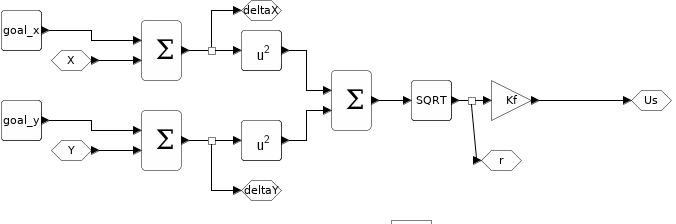
\includegraphics[scale = 0.5]{images/Us_model.png} }

	\caption{Схема получения сигнала $U_{s}$}
	\label{fig:Us}
\end{figure}  
    
\item Cхема получения сигнала $U_{rotation}$.

\begin{figure}[h!]
	\centering{ 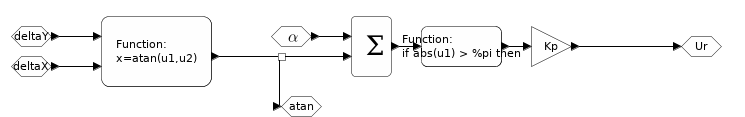
\includegraphics[scale = 0.5]{images/Ur_model.png} }

	\caption{Схема получения сигнала $U_{r}$}
	\label{fig:Ur}
\end{figure} 

В данной схеме стоит заметить, что в одном из блоков используется математическая функция $atan$, возвращающая значения $(-\pi; \pi]$. В тех случаях, когда роботу надо развернуться на 180 градуов или приблизительно на данный угол, функция начинает возвращать значения резко скачущие в пределах $(-\pi; \pi]$, что заставляет робота постоянно менять направление своего движения (рис.  ~\ref{fig:Atan_coord}). Данную проблему можно решить, добавив блок с кодом на рис. ~\ref{fig:Pi_mod}.

 \begin{figure}[h!]
	\centering{ 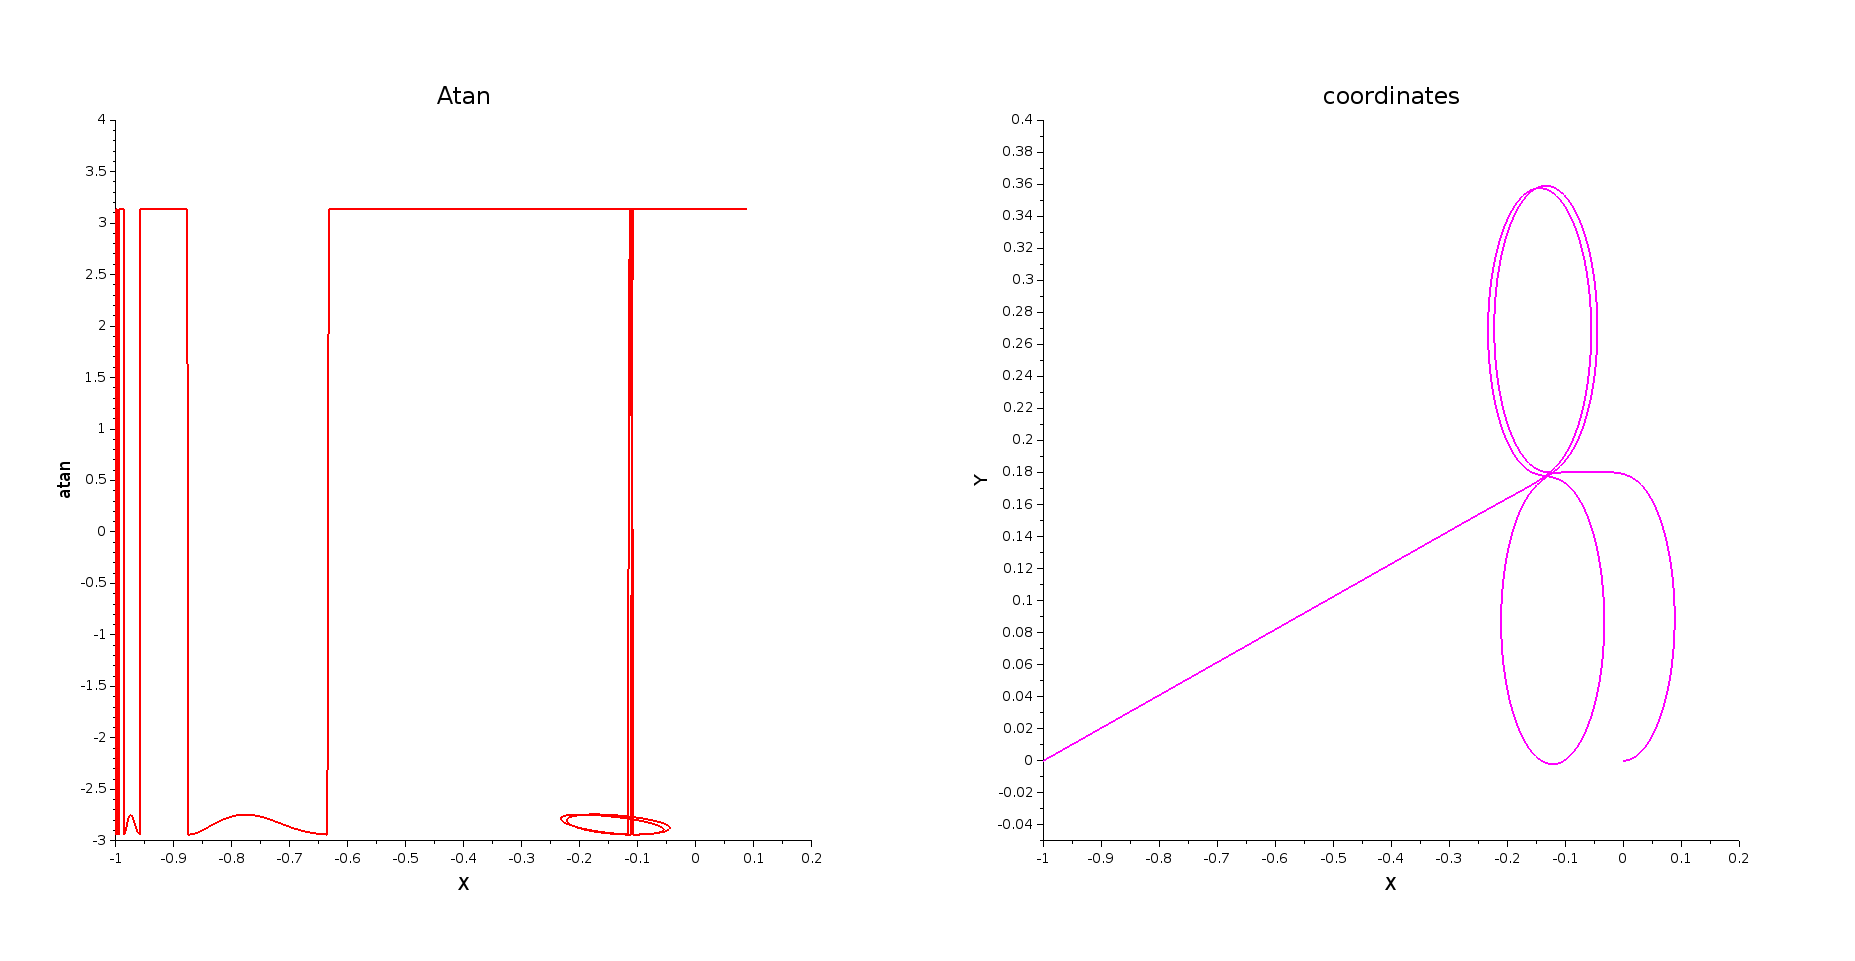
\includegraphics[scale=0.2]{images/Atan_coord.png} }
    \caption{Значения возвращаемые функцией $atan$ и траектория движения робота в точку $(-1;0)$.}
	\label{fig:Atan_coord}
\end{figure} 

 \begin{figure}[h!]
	\centering{ 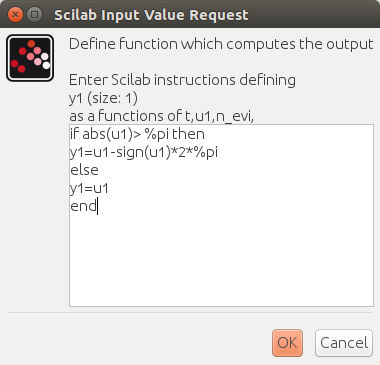
\includegraphics[scale=0.5]{images/Pi_mod_window.png}}
    \caption{Код для решения проблемы $atan$.}
	\label{fig:Pi_mod}
\end{figure} 

После включения этого блока, мы получим следующую траекторию (рис. ~\ref{fig:New_trajectory}) для тех же координат.

Также при задании некоторых координат, программа зависает. Решением данной проблемы будет ввод в блок арктангенса дополнительного условия (рис. ~\ref{fig:Atan_window})

\begin{figure}[h!]
\begin{center}
    \begin{minipage}[h]{0.4\linewidth}
    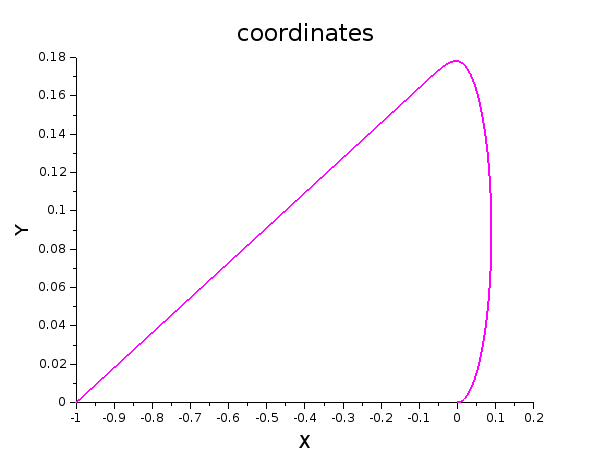
\includegraphics[width=1\linewidth]{images/New_trajectory.png}
    \caption{Исправленная траектория.}
	\label{fig:New_trajectory}
    \end{minipage}
    \hfill
    \begin{minipage}[h]{0.4\linewidth}
    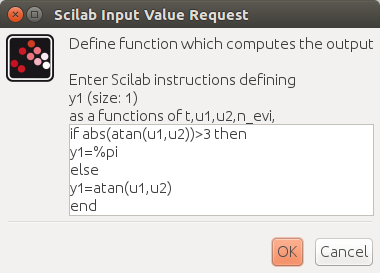
\includegraphics[width=1\linewidth]{images/Atan_window.png}
    \caption{Окно блока $atan$.}
	\label{fig:Atan_window}
    \end{minipage}
\end{center}
\end{figure}

\item Схема подачи сигнала на двигатели и получения угловых скоростей. Модель двигателей следует взять из лабораторной работы 2. (рис. ~\ref{fig:Engiens}).


\item Схема расчёта угла поворота робота (рис. ~\ref{fig:steering_angle}).

\begin{figure}[h!]
\begin{center}
    \begin{minipage}[h]{0.4\linewidth}
    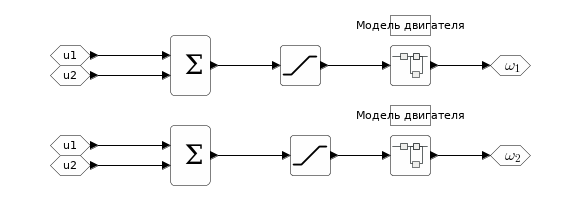
\includegraphics[width=1\linewidth]{images/Engiens.png}
    \caption{Модель двигателей EV3.}
    \label{fig:Engiens}
    \end{minipage}
    \hfill
    \begin{minipage}[h]{0.4\linewidth}
    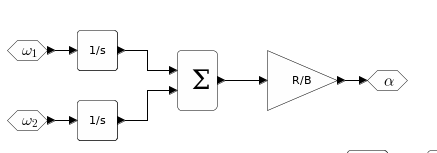
\includegraphics[width=1\linewidth]{images/angle.png}
    \caption{Схема получеия угла поворота.}
    \label{fig:steering_angle}
    \end{minipage}
\end{center}
\end{figure}

\item Схема получения текущих координат робота (рис. ~\ref{fig:Coord}).

 \begin{figure}[h!]
	\centering{ 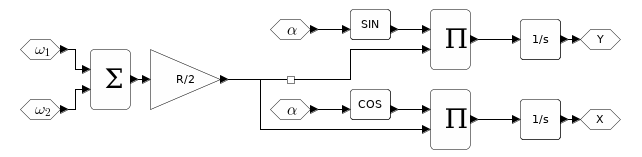
\includegraphics[scale=0.5]{images/Coordinates.png}}
    \caption{Схема получения координат.}
	\label{fig:Coord}
\end{figure} 

\end{enumerate}

\section{Цель работы}
Получить опыт построения математической модели робота, освоить алгроитм движения робота с дифференциальным приводом к заданной точке.
\section{Порядок выполнения работы}
\begin{enumerate}
\item Собрать робота-машинку, контрукционно схожим с роботом в лабораторных работах 3 или 4, но без каких-либо установленных датчиков.
\item Создать модель в Xcos, используя схемы п. ~\ref{par:Xcos}. 
\item Написать программу на языке python3, которая будет удовлетворять разделу "Описание задания работы", и подобрать значение коэффициентов для пропорционального регулятора
\item Снять данные x и y робота для нескольких координат. Предлагается выбрать точки в разных координатных плоскостях, а также на осях координат. 
\item Написать программу в Scilab для построения траектории робота.
\item Построить траектории, полученные с модели и с реального робота, в одной координатной плоскости. Они должны совпадать полностью или с небольшими отклонениями. Пример рис.~\ref{fig:trajes}
\end{enumerate}
\begin{figure}[h!]
	\centering{ 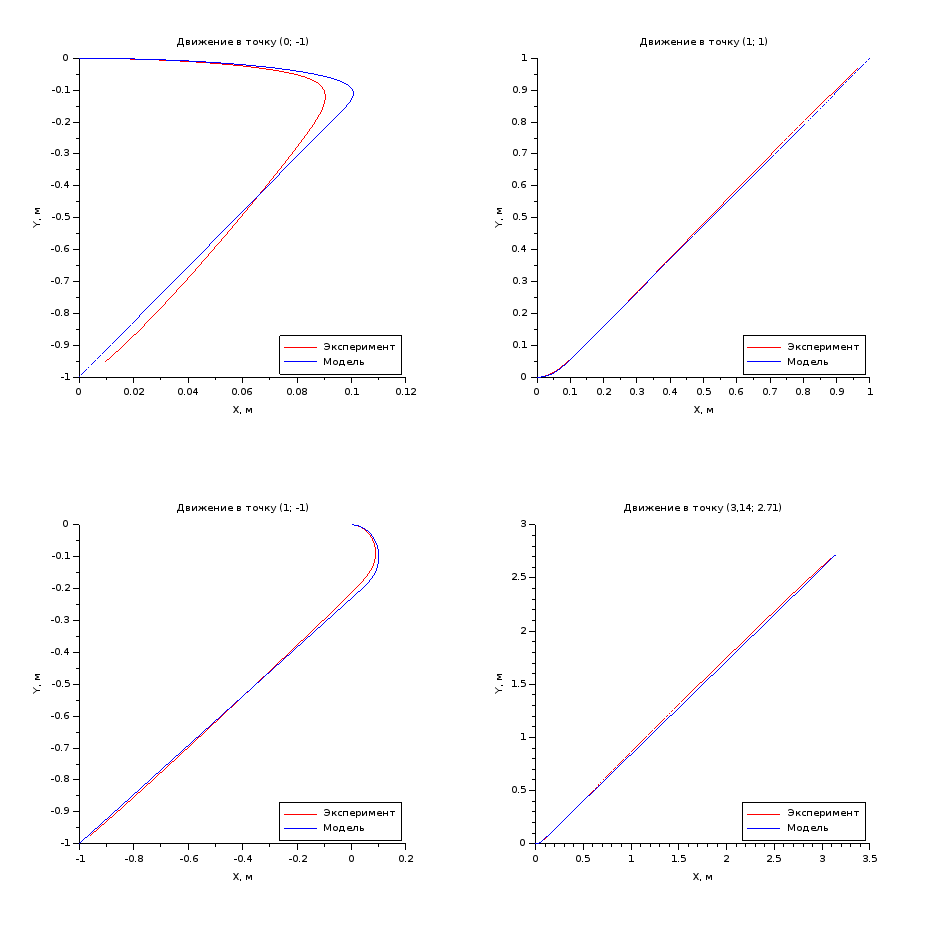
\includegraphics[scale=0.5]{images/plots_lab5.png}}
    \caption{Примеры полученных траекторий.}
	\label{fig:trajes}
\end{figure} 

\newpage
\section*{Приложение А\\
Пример подходящего для экспериментов робота-машинки.}
\vspace{1cm}
\begin{figure}[h!]
	\centering{ 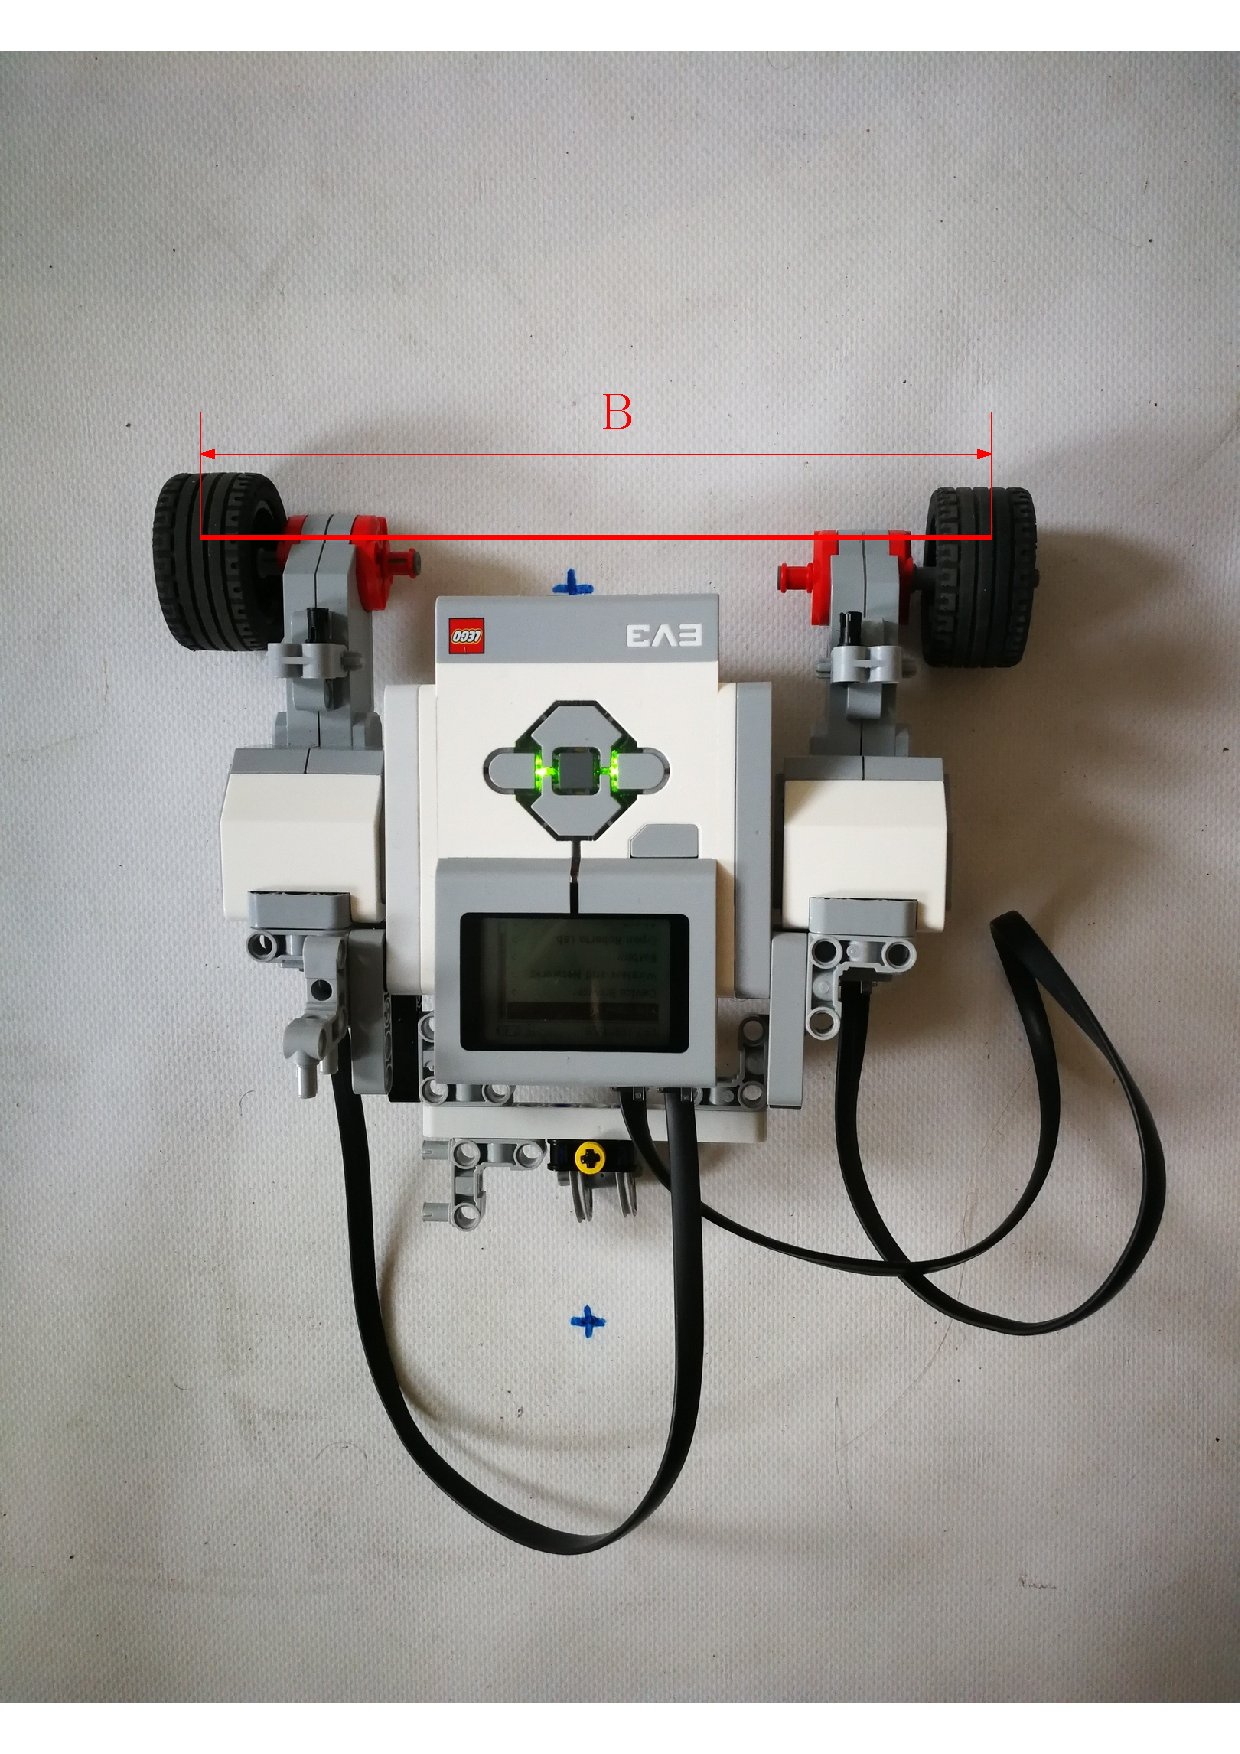
\includegraphics[width=16cm]{robot.pdf} }
	\vspace{-0.5cm}
	\caption{Робот с обозначением колесной базы}
	\label{fig:first_append_fig}
\end{figure}	

\end{document}
